\documentclass{article}

%% Page Margins %%
\usepackage{geometry}
\geometry{
    top = 0.75in,
    bottom = 0.75in,
    right = 0.75in,
    left = 0.75in,
}

\usepackage{amsmath}
\usepackage{graphicx}
\usepackage{tikz}
\usepackage{parskip}

\title{CSC209 Project}

\author{Samuel Iacobazzi}

\begin{document}
\maketitle

5.1 Overview
\newline This project seeks to implement a simple shell with some basic features. This is obviously interactive and user input and output are done through the terminal. 
Key features include switching the current directory and piping processes together.
\newline\newline
5.2 Building
\newline The project can be build with ``make'', and can be run with ``./netsh.elf''. 
\newline\newline
5.3 Architecture
\newline The downward arrows indicate forks from the parent, and the other arrows indicate pipes from one child to the next, ultimately back to the parent shell.
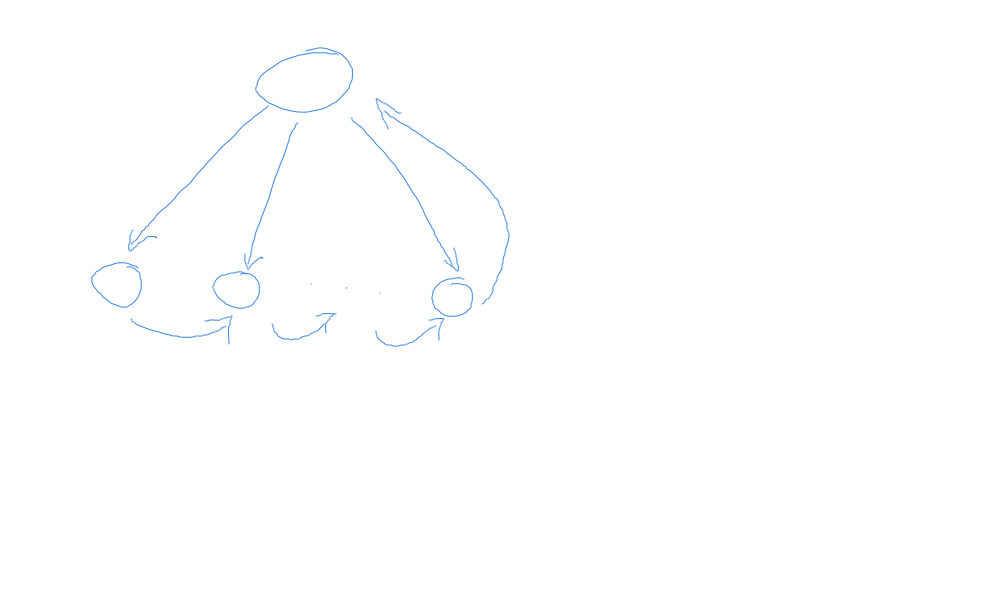
\includegraphics[scale=0.5]{model.png}
\newline\newline
5.4 Communication
\newline Communication was extremely simple to implement in this project since it sufficed to take maximum advantage of the kernel's services; 
automatic blocking on pipe reads and programs waiting for EOF or special characters were enough to be able to avoid special signaling.
\newline\newline
5.5 Concurrency
\newline This was similarly straightforward; if multiple programs are piped together, the shell creates a doubly linked list to serve as a job queue, 
then allocates pipes between each to-be process, then simply forks them all in a loop and waits for the last child to die.
\newline\newline
5.6 Error Handling
\newline The only forseeable adversarial errors are malformed commands or path variable manipulation; i.e. a user could place random pipes in the input, give 
an invalid program name, or, again, tamper with the path variable. These are handled simply by throwing an error message depending on the issue and returning to the prompt.

\end{document}